\section{Nearest Neighbor and Integral Image}\label{sec:nnii}


In this section, we overview the desired functionality of nearest neighbor, 
integral Image functions at a higher level implementation and their scope 
for parallelization on a GPU in tandem. Next, we discuss their kernel 
level implementation details and strategies employed.

\subsection{Nearest Neighbor (NN)}\label{sec:nn}

We have seen the significance of downscaling in the background of image 
pyramid, to make the face detection independent of the detection window size.  
The downscaled image is calculated by the nearest neighbor function. 
Every time the image’s width and height are downscaled by a factor 
of 1.2 until one of them reaches the detection window’s width or height of 25 pixels. 
Figure~\ref{fig:NN} shows the nearest neighbor output  with 
scaling factor of 2 on a source image of 8 X 8 pixels
\textit{(relate to final image pixels in the source using red color coding)}.

\begin{figure}[h]
  \centering
  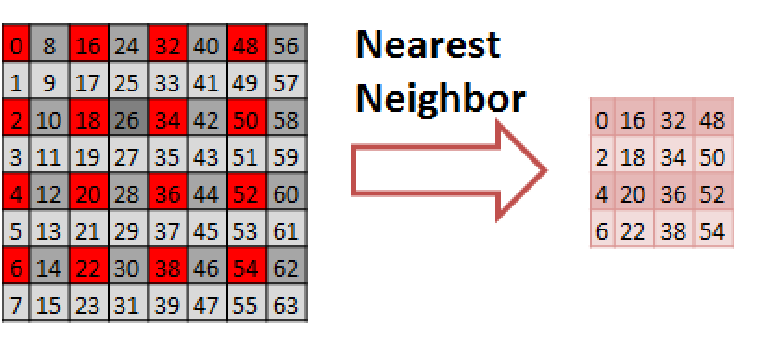
\includegraphics[width=0.9\linewidth]{figs/nn_img_crop.pdf}
  \caption{Image downscaling using nearest neighbor}
  \label{fig:NN}
\end{figure}

\paragraph{Parallelization Scope}
we can see that each pixel in the downscaled image can be calculated 
by scale factor offset,  width and  height of the source image. 
So we map each (or more) pixel positions to be fetched 
by a single thread. Here, we map two pixels each separated 
by a block dimension, to each thread.


\subsection{Integral Image (II)}\label{sec:II}

For each X  \& Y in the downscaled image, Integral Image computes 
the sum of all the pixels above \& to the left of (X, Y).  We split 
it into two separate operations as RowScan(RS) and columnScan(CS) of the 
image, where, RowScan(RS) is inclusive prefix scan along the row for all 
the rows and ColumnScan(CS) is inclusive prefix scan along the column for all the columns.
Figure~\ref{fig:II} shows the output image generated for RS and CS implementation 
on a downscaled image
\textit{(relate to the integral sum of highlighted pixels in source with the pixel value '36' in final image)}.

\begin{figure}[h]
  \centering
  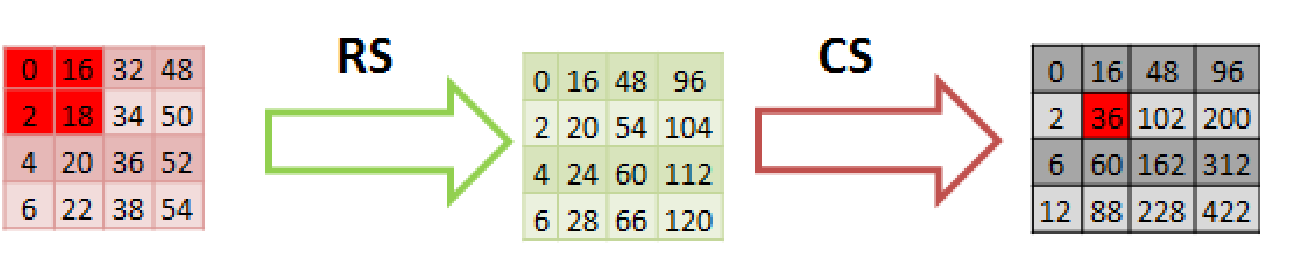
\includegraphics[width=\linewidth]{figs/ii_img_crop.pdf}
  \caption{Image integral sum calculation }
  \label{fig:II}
\end{figure}



\paragraph{Parallelization Scope}
In RowScan, prefix scan of each row is independent of the other rows 
in the image and same is the case with columns in the ColumnScan operation. 
So we can leverage the block level parallelism here. Prefix scan for a row/column  
by itself seems to be a sequential operation, but we can paralleize that too !!
\textit{(discussed in kernel implementation)}.

Similarly we compute the square integral sum \textit{(integral sum of the squared pixel values)}
for doing the variance. We need the variance of the pixels for the haar rectangle co-ordinates, 
in the Cascade classifier stage. Variance can be determined 
as \textit{Var(X) = E(X\textsuperscript{2}) - (E(X)*E(X))
where, E(X) is the mean(here, integral sum) 
and E(X\textsuperscript{2}) is the mean of X squared(here, square integral sum)}.



\subsection{Implementation of Nearest Neighbor and Integral Image}\label{sec:impl nn II}
The implementation of nearest neighbor and integral Image\textit{(RowScan(RS) \& ColumnScan(CS)) } was 
split into four separate kernels as below.

\vspace{0.1in}
\begin{itemize}
\item \textit{Kernel 1} \begin{math}\rightarrow\end{math} Nearest Neighbor(NN) \& RowScan (RS)- downscaled image ready
\item \textit{Kernel 2} \begin{math}\rightarrow\end{math} Matrix Transpose
\item \textit{Kernel 3} \begin{math}\rightarrow\end{math} RowScan
\item \textit{Kernel 4} \begin{math}\rightarrow\end{math} Matrix Transpose
\end{itemize}

Integral sum \& square integral sum are ready at the end of kernel 4. ColumnScan itself is broke down as Kernels 2, 3 and 4. 

\paragraph{Kernel 1 - Nearest Neighbor(NN) \& RowScan(RS)}
We accomplish the nearest neighbor and rowscan functionality 
in a single kernel to avoid storing the downscaled image to 
global memory between kernel launches. Instead, we store 
each downsampled row of the source image in the shared memory 
and call the \textit{‘\_\_syncthreads()\_\_’} function before we proceed to 
RowScan on that respective row. Effectively we eliminate a global 
memory read of the down scaled image. we used the Harris-Sengupta-Owen 
algorithm to parallelize the RowScan operation within each row. 
Figure~\ref{fig:kernel1} walks you through the flow of this kernel.

\begin{figure}[h]
  \centering
  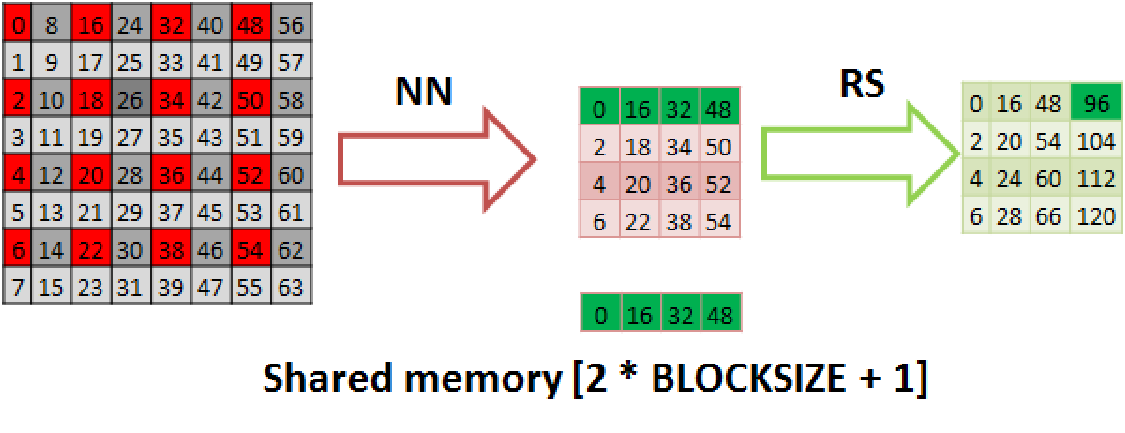
\includegraphics[width=\linewidth]{figs/kernel1_crop.pdf}
  \caption{Kernel1: NN \& RS }
  \label{fig:kernel1}
  \end{figure}

\paragraph{Kernels 2, 3 \& 4 - ColumnScan(CS)}
First we transpose the image matrix output of Kernel 1, then do a 
RowScan on it and finally transpose it back to obtain the integral Image sum. 
Effectively, the Kernels 2,3 \& 4 together form the CoumnScan operation. 
Let’s analyze the rationale behind this split up. In a straightforward 
implementation of ColumnScan, each thread brings the first element in each row of 
the image matrix to the shared memory and does a inclusive prefix scan on it. 
Figure~\ref{fig:cs_impl} shows the access pattern in the image matrix and 
Figure~\ref{fig:gm_layout} gives the corresponding global memory layout.

\begin{figure}[h]
  \centering
  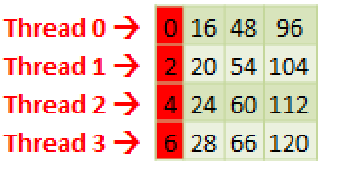
\includegraphics[width=0.4\linewidth]{figs/img_matrix_crop.pdf}
  \caption{Image matrix data access in ColumnScan }
  \label{fig:cs_impl}
\end{figure}

\begin{figure}[h]
  \centering
  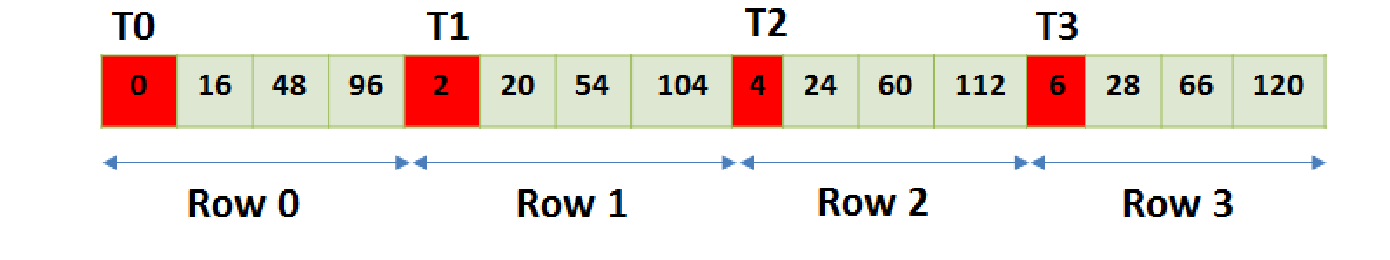
\includegraphics[width=\linewidth]{figs/global_mem_crop.pdf}
  \vspace{0.05in}
  \caption{Global memory layout of the Image matrix }
  \label{fig:gm_layout}
\end{figure}

We see from Figure~\ref{fig:gm_layout} that global memory reads aren’t coalesced. Each access to 
global memory takes about 400 – 500 cycles and every thread needs separate 
access in this case. So we bypass this problem by splitting the ColumnScan 
into kernels 2,3 \& 4 where each of them does a coalesced global memory read/write. 
Figure~\ref{fig:cs_brkdwn } shows the columnScan functionality broken down and implemented in three separate kernels. 

\begin{figure*}[h]
  \centering
  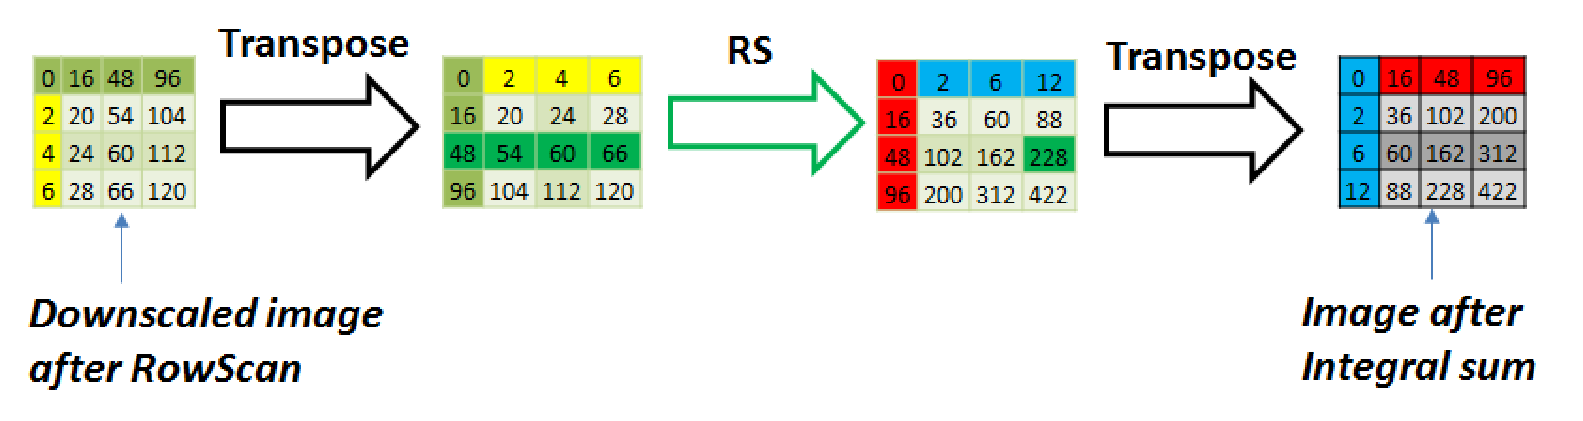
\includegraphics[width=0.85\linewidth]{figs/cs_break_crop.pdf}
  \caption{ColumnScan kernel breakdown }
  \label{fig:cs_brkdwn }
\end{figure*}


